\chapter{SPQR trees}

Before we show another interesting structure called SPQR-trees note that they are not related to the previously mentioned PQ-trees. Also in this section we will be considering multigraphs without loops, i.e. graphs can have parallel edges.

\begin{defn}
	Let $G = (V_G, E_G)$ be a biconnected multigraph, a \textbf{skeleton} of $G$ is multigraph $H = (V_H, E_H)$ with these properties:
	
	\begin{enumerate}
		\item $V_H \subseteq V_G$;
		\item every edge $e = \{u,v\} \in E_H$ represents a connected subgraph $G_e$ of $G$ ("pertinent graph of $e$") which contains the vertices $u,v$;
		\item every edge of $G$ belongs to exactly one pertinent graph;
		\item for $e,f \in E_H, e \neq f$, then $V(G_e) \cap V(G_f) = e \cap f$.
	\end{enumerate}
\end{defn}

\begin{figure}[!ht]\centering
	\begin{subfigure}{.3\textwidth}\centering
		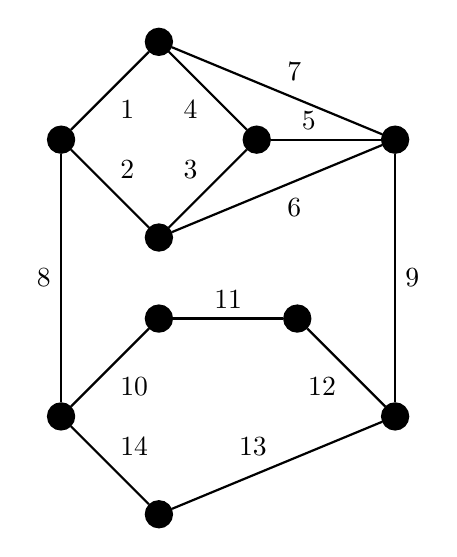
\begin{tikzpicture}[node distance = 50, main/.style = {draw, circle, fill}, thick]
			\node[main] (1) {};
			\node[main, above right of = 1] (2) {};
			\node[main, below right of = 1] (3) {};
			\node[main, above right of = 3] (4) {};
			\node[main, right of = 4] (5) {};
			\node[below of = 1] (p1) {};
			\node[main, below of = p1] (6) {};
			\node[below of = 5] (p5) {};
			\node[main, below of = p5] (7) {};
			\node[main, above right of = 6] (8) {};
			\node[main, above left of = 7] (9) {};
			\node[main, below right of = 6] (10) {};
			\draw (1) -- (2) node[midway, below right] {1};
			\draw (1) -- (3) node[midway, above right] {2};
			\draw (3) -- (4) node[midway, above left] {3};
			\draw (2) -- (4) node[midway, below left] {4};
			\draw (4) -- (5) node[midway, above left] {5};
			\draw (3) -- (5) node[midway, below right] {6};
			\draw (2) -- (5) node[midway, above right] {7};
			\draw (1) -- (6) node[midway, left] {8};
			\draw (5) -- (7) node[midway, right] {9};
			\draw (6) -- (8) node[midway, below right] {10};
			\draw (8) -- (9) node[midway, above] {11};
			\draw (7) -- (9) node[midway, below left] {12};
			\draw (7) -- (10) node[midway, above left] {13};
			\draw (6) -- (10) node[midway, above right] {14};	
		\end{tikzpicture}
	\end{subfigure}
	\begin{subfigure}{.3\textwidth}\centering
		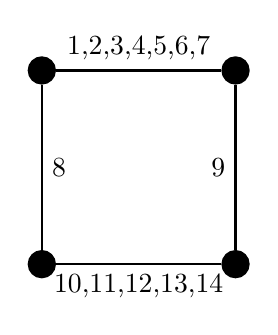
\begin{tikzpicture}[node distance = 70, main/.style = {draw, circle, fill}, thick]
			\node[main] (1) {};
			\node[main, left of = 1] (2) {};
			\node[main, below of = 1] (3) {};
			\node[main, below of = 2] (4) {};
			\draw (1) -- (2) node[midway, above] {1,2,3,4,5,6,7};
			\draw (1) -- (3) node[midway, left] {9};
			\draw (2) -- (4) node[midway, right] {8};
			\draw (3) -- (4) node[midway, below] {10,11,12,13,14};
		\end{tikzpicture}
	\end{subfigure}
	\begin{subfigure}{.3\textwidth}\centering
		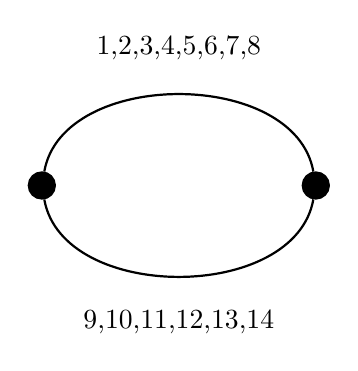
\begin{tikzpicture}[node distance = 70, main/.style = {draw, circle, fill}, thick]
			\node[main] (1) {};
			\node[above right of = 1] (l1) {1,2,3,4,5,6,7,8};
			\node[below right of = 1] (l2) {9,10,11,12,13,14};
			\node[main, below right of = l1] (2) {};
			\draw[bend left = 80] (1) edge (2);
			\draw[bend right = 80] (1) edge (2);
		\end{tikzpicture}
	\end{subfigure}
	\caption{Example of graph $G$ and some of its skeletons.}
\end{figure}

\begin{defn}
	\textbf{Separation tree $T$} of a biconnected $G = (V_G, E_G)$ is a tree whose leaves correspond bijectively to edges of $G$, every internal node $\alpha$ has degree $\geq 3$ and has an associated skeleton $S_\alpha$ of $G$ with $\deg(\alpha)$ edges, such that the edge sets of the pertinent graphs of $S_\alpha$ correspond to the sets of leaves in the components of $T - \alpha$.
\end{defn}

\begin{defn}[SPQR-tree]
	An SPQR-tree of a biconnected multigraph is a separation tree $T$ whose internal nodes are of three types:
	
	\begin{enumerate}
		\item S-nodes (series): nodes whose skeleton is a cycle of length $\geq 3$.
		\item P-nodes (parallel): nodes whose skeleton is a graph with 2 vertices and $\geq 3$ parallel edges.
		\item R-nodes (ridged): nodes whose skeleton is a simple 3-connected graph.
	\end{enumerate}
	
	\noindent Moreover, no two S-nodes are adjacent and also no two P-nodes are adjacent. Sometimes Q-node is referred as leaf.
\end{defn}

\begin{fact}
	Every biconnected multigraph has unique SPQR-tree which can be computed in linear time.
\end{fact}

\begin{thm}
	Let $G$ be a biconnected multigraph with $m$ edges, $m \geq 3$, let $T$ be a separation tree of $G$. Then all the skeletons in $T$ have together at most $3m-6$ edges.
\end{thm}

\begin{proof}
	By induction on $m$. For $m = 3$ we have only one type of SPQR tree which is a tree with one internal node and three nodes. In the internal node there can either be a triangle or three-parallel edges graph. But in both case we have that $3m - 6 = 9 - 6 = 3$ which is true.
	
	Let $m > 3$ and consider case 1: $T$ has a single internal node, then it is also fine. Case 2 consider that $T$ has 2 adjacent internal nodes $\alpha, \beta$ and $|E_\alpha| \geq 2, |E_\beta| \geq 2$. Split $G$ into: $G_\alpha$ which is formed by $E_\alpha$ plus new edge $uv$, similarly $G_\beta$ which is formed by $E_\beta$ plus new edge $uv$. Where $u$ and $v$ are the split vertices between $\alpha$ and $\beta$. From these we create their separation trees, which will be made by "replacing" the second vertex by a leaf representing edge $uv$.
	
	By "disconnecting" edge $\alpha\beta$ in $T$ we obtain separation trees $T_\alpha, T_\beta$ for $G_\alpha, G_\beta$ respectively. Let $k := |E_\alpha|, m -k := |E_\beta|$ and $G_\alpha$ has $k+1$ edges and $G_\beta$ has $m-k+1$ edges.
	
	Finally use induction. Skeletons in $T_\alpha$ have at most $3(k+1)-6$ edges and skeletons in $T_\beta$ have at most $3(m-k+1)-6$ edges. Therefore skeletons in $T$ have at most $3k + 3 - 6 + 3m - 3k + 3 - 6 = 3m -6$ edges.
\end{proof}

\section{Create SPQR tree}

In this section we will show some techniques how an SPQR tree can be constructed.

\begin{defn}
	Suppose $G = (V_G, E_G)$ is a biconnected multigraph, $uv \in V_G, u \neq v$, edges $e,f \in E_G$ are in the same separation class w.r.t. $uv$ (that is $e \sim_{uv} f$) if
	
	\begin{enumerate}
		\item $e = f$;
		\item there is a path containing $e$ and $f$ whose internal vertices are different from $u,v$;
		\item there is a cycle containing $e$ and $f$ and containing at most one of $u,v$.
	\end{enumerate}
\end{defn}

\begin{fact}
	$\sim_{uv}$ is an equivalence on $E_G$.
\end{fact}

\begin{defn}
	$u,v$ are separation pair if $\sim_{uv}$ has more than one classes.
\end{defn}

We may see that cuts are separation pairs, but in fact not the only. For example $K_4$.

\begin{defn}
	A separation pair is \textbf{trivial} if
	
	\begin{enumerate}
		\item $\sim_{uv}$ has two classes, one of them contains just an edge
		\item $\sim_{uv}$ has 3 classes, all of them contains just one edge.
	\end{enumerate}
\end{defn}

\begin{observ}
	If $G$ has non-trivial separation pair, then $G$ is one of the following graphs: two vertices with two parallel edges, two vertices with three parallel edges, triangle, any simple 3-connected graph.
\end{observ}

\noindent Now we will show how to find an SPQR tree:

\begin{enumerate}
	\item Start with one internal node having entire $G$ in it and $|E_G|$ leaf nodes.
	\item As long as any skeleton has non-trivial separation pair $uv$ then split skeleton along $uv$.
	
	\begin{itemize}
		\item Splitting skeleton $S = (V_S, E_S)$ along a non-trivial separation $uv$. Firstly partition $E_S$ into two parts $E_{I}, E_{II}$ s.t. each part has at least two edges and each part is a union of $\sim_{uv}$-classes.
	\end{itemize}
	
	\item Merge adjacent P-nodes and S-nodes.
	
	\begin{itemize}
		\item When we have two S-nodes then we have two circles where one edge is representing the other graph of the second node. So together they form one circle. For P-nodes we have some parallel edges in between two vertices, where one is for the other part of the graph. Thus all together it is all of their parallel edges together.
	\end{itemize}
\end{enumerate}

\noindent This procedure will lead to SPQR tree.

\section{SPQR-trees and planarity}

We remind ourselves what a planar embedding of a connected graph is: rotation scheme (which is the cyclic order of edges around vertex).

\begin{thm}
	A biconnected $G$ is planar \ifft every skeleton in its SPQR-tree is planar $\iff$ every R-skeleton is planar.
\end{thm}

\begin{proof}
	"$\Rightarrow$" $K$ is a skeleton of $G \Rightarrow G$ has a subdivision of $K$ as a subgraph. Thus $K$ has to be planar.
	
	"$\Leftarrow$" We have embedding for all skeletons. Choose arbitrary root of SPQR-tree and process from bottom to top. For every edge of every skeleton other than the edge corresponding to the parent: construct the embedding of its pertinent graph, where the poles are in the same face (poles are the two special vertices). For vertex representing a skeleton: ignore the edge of a parent and combine the children to the current skeleton.
\end{proof}

\begin{defn}
	$G$ biconnected graph with SPQR-tree $T$, $K$ skeleton of $T$, $\mathcal{G}$ embedding of $G$, $\mathcal{K}$ embedding of $K$, $\mathcal{G}$ is \textbf{consistent} with $\mathcal{K}$ if
	
	\begin{enumerate}
		\item For every edge $e = \{x,y\} \in E(K)$, the edge of $G_e$ (pertitent graph of $e$) incident to $x$ form a cyclic interval in the rotation scheme $x$ in $\mathcal{G}$, same for $y$.
		\item For $e,f,g \in E(K)$ meeting in $x$, for $e' \in G_e, f' \in G_f, g' \in G_g$ meeting in $x$ the order of $e,f,g$ in $\mathcal{K}$ is the same as the order of $e',f',g'$ in $\mathcal{G}$.
	\end{enumerate}
\end{defn}

\begin{thm}
	$G,T$ as above, then
	
	\begin{enumerate}
		\item For every embedding $\mathcal{G}$ of $G$ each skeleton in $T$ has unique embedding consistent with $\mathcal{G}$.
		\item For any choice of an embedding of each skeleton of $T$, $G$ has unique embedding consistent with all skeletons.
	\end{enumerate}
\end{thm}

\begin{proof}
	We will showcase both properties.
	
	\begin{enumerate}
		\item We have $\mathcal{G}$ embedding of $G$ and skeleton $K$.
		
		\begin{enumerate}
			\item Firstly consider $x$ is not an articulation, since $G$ and $K$ are biconnected thus they have to be paths to $y$. We have 4 paths from $x$ to $y$ either $f_1, f_2$ are in the same pertinent which is not possible since they would meet in vertex of $K$, or if they are different from P-skeleton, then it is R (ridgit) thus there would be the path. Which is a contradiction. Thus it is P-skeleton. Hence the first part of the definition is done.
			
			\item Due to the cyclic intervals for $e,f,g \in E(K)$ they form a cyclic intervals. To show that it forms an embedding choose a path representing in its edge in $K$ and draw it.
		\end{enumerate}
	
		\item Fix an embedding of every skeleton. There exist one embedding that was constructed like in the previous theorem and we have two embeddings of $\mathcal{G}$ s.t. $\mathcal{G} \neq \mathcal{G}'$ so one cyclic order differs. We have to find node where $e',f',g'$ are in different pertinent. We may find an internal node which separates $e',f',g'$ so it suffices what we were looking for. So due 2. only one $\mathcal{G}$ or $\mathcal{G}'$ can be consistent.
	\end{enumerate}
\end{proof}

\begin{note}
	S-skeleton has exactly 1 embedding. R-skeleton has exactly 2 embeddings. P-skeletons with $m$ edges has $(m-1)!$ embeddings.
\end{note}

\noindent We can have more restricitions or we may count how many embeddings given graph has.

\begin{mybox}{Partially Embedded Planarity (or PEP for short)}
	\begin{itemize} []
		\item \textbf{Input:} graph $G = (V_G, E_G)$, subgraph $H = (V_H, E_H)$, embedding $\mathcal{H}$ of $H$.
		\item \textbf{Output:} Is there a way to extend $\mathcal{H}$ into an embedding of $G$?
	\end{itemize}
\end{mybox}

\begin{rem}
	This is a special example of general cases such that partially representation is given and we have to construct the whole representation.
\end{rem}

\begin{note}
	Embedding of $H$ is given by
	
	\begin{enumerate}
		\item rotation scheme
		\item for every cycle $C$ on the boundary of a face of $\mathcal{H}$ on every vertex $x \notin C$, specify on which side of $C$ $x$ is drawn. -- \textit{"cyclic-vertex position"}
	\end{enumerate}

	Note that again it does not keep the information about the outer face.
\end{note}

\begin{thm}
	PEP can be solved in polynomial (in fact linear) time.
\end{thm}

\begin{proof}
	Assume $G$ is biconnected. Then see this algorithm.
	
	\begin{algorithm}[!ht]
		\begin{algorithmic}[1]
			\State Compute SPQR-tree of $G$. This can be uniquely computed in linear time.
			\If{$G$ is not planar}
				\State \Return
			\EndIf
			\ForAll{skeletons}
				\State Determine whether it can be embedded in not obviously wrong way or have a counter example.
			\EndFor
		\end{algorithmic}
	\end{algorithm}

	\begin{defn}
		Let $K$ be a skeleton of the SPQR tree of $G$, an embedding $\mathcal{K}$ of $K$ is \textbf{obviously wrong} if
		
		\begin{enumerate}
			\item $\mathcal{H}$ has three edges $e,f,g$ meeting in a single vertex $x$, $\mathcal{K}$ has three edges $\bar{e}, \bar{f}, \bar{g}$, each having one of $e,f,g$ in its pertinent graph, the cyclic order of $e,f,g$ in $\mathcal{H}$ differs from the cyclic order if $\bar{e}, \bar{f}, \bar{g}$ in $\mathcal{K}$.
			\item $\mathcal{H}$ has facial cycle $C$ and a vertex $x \notin V(C)$, the edges of $C$ projects to more then one pertinent graph of $K$, hence the edges of $K$ into which the edges of $C$ projects form a cycle $\bar{C}$, and $x$ is in the pertinent graph of an edge $\bar{E} \notin V(\bar{C})$, and in $\mathcal{K}$ the edge $\bar{e}$ is on the wrong side of $\bar{C}$. 
		\end{enumerate}
	\end{defn}

	\begin{observ}
		If a skeleton $K$ is embedded in obviously wrong way, then the embedding $\mathcal{G}$ of $G$ induced by the skeletons does not extend $\mathcal{H}$.
	\end{observ}

	\begin{thm}
		If every skeleton of the SPQR-tree of $G$ is embedded in a way that is not obviously wrong, then the embedding $\mathcal{G}$ of $G$ induced by these skeleton embeddings extends $\mathcal{H}$.
	\end{thm}

	\begin{proof}
		For the two rules if they are satisfied then the extension is rather straightforward. That is if we have some cyclic order in $\mathcal{H}$ we just insert new edges in between to the new cyclic order in $\mathcal{G}$. For the outer vertex $x$ outside cycle $C$ it is even easier.
		
		But suppose that the first rule is not satisfied. Then in SPQR tree is unique node having three leaves in different part. This node and particularly its skeleton must have been obviously wrong.
		
		Now if the second rule is note satisfied then take path from $x$ towards $\bar{C}$. $y \in \bar{C}$ first met and $e,f \in \bar{C}$ having $y$ as one vertex and $g \notin \bar{C}$ be the last edge of the path. Find separation node. Let $x\in \bar{e} \notin \bar{C}$ where $\bar{e}$ is skeleton edge and $\bar{C}$ cycle in the skeleton of $C$. Then this $\mathcal{K}$ is obviously wrong embedding.
	\end{proof}

	\begin{thm}
		There is a polynomial algorithm which for a given $\mathcal{H}$ and SPQR-tree skeleton $K$ of $G$ determines whether $K$ has an embedding which is not obviously wrong.
	\end{thm}

	\begin{proof}
		\begin{enumerate}[I)]
			\item If $K$ is S-skeleton: it has 1 embedding, which is never obviously wrong.
			\item If $K$ is R-skeleton: it has 2 embeddings, so we just check the properties for both possible embeddings.
			\item If $K$ is P-skeleton with $d \geq 3$ edges: it has $(d-1)!$ embeddings. Do the following. $E_{xy} :=$ edges of $K$ which contains edge of $H$ incident ot $x$ and also edge of $H$ incident ot $y$ in their pertinent graph.
			
			\begin{enumerate}[1.]
				\item Determine cyclic order of $E_{xy}$ that is not obviously wrong.
				\item Insert into the cyclic order of $E_{xy}$ edges having an edge of $\mathcal{H}$ incident to $x$ or $y$, in a way that is not obviously wrong.
				\item For edge if $K$ that contains no edge of $\mathcal{H}$ incident to $x$ or $y$ in its pertinent graph: insert it in a way that is not obviously wrong (if possible).
			\end{enumerate}
		
			Note that if constraint related to cycle vertex position affects me, then it is because of a cycle $\bar{C}$ in $K$ where both edges pf $\bar{C}$ are in $E_{xy}$.
		\end{enumerate}
	\end{proof}
\end{proof}